\documentclass[a4paper, 12pt, titlepage]{article}
\usepackage[utf8]{inputenc}
\usepackage[english]{babel}
\usepackage[]{parskip}
\usepackage{graphicx}
\usepackage{xcolor}
\usepackage{paralist} % compactitem
\usepackage{csquotes}
\usepackage{wrapfig}
\usepackage{subfig}
\usepackage{csvsimple} % csv tables

% Title spacing
\usepackage{titlesec}
\titlespacing*{\section}{0pt}{0pt}{0pt}
\titlespacing*{\subsection}{0pt}{-5pt}{-5pt}
\titlespacing*{\subsubsection}{0pt}{0pt}{0pt}

% Citations
\usepackage[
  style=ieee,
  citecounter,
  labelnumber,
  backend=biber,
  bibencoding=utf8,
  sorting=none
]{biblatex}
\addbibresource{references.bib}

% Code blocks
\usepackage{listings}
\definecolor{codegreen}{rgb}{0,0.6,0}
\definecolor{codegray}{rgb}{0.5,0.5,0.5}
\definecolor{codepurple}{rgb}{0.58,0,0.82}
\definecolor{backcolour}{rgb}{1.0,1.0,1.0}
\lstdefinestyle{mystyle}{
  backgroundcolor=\color{backcolour},
  commentstyle=\color{codegreen},
  keywordstyle=\color{magenta},
  numberstyle=\tiny\color{codegray},
  stringstyle=\color{codepurple},
  basicstyle=\ttfamily\tiny,
  breakatwhitespace=false,
  breaklines=true,
  captionpos=b,
  keepspaces=false,
  numbersep=5pt,
  showspaces=false,
  showstringspaces=false,
  showtabs=false,
  tabsize=2
}
\lstset{style=mystyle}

% Custom commands
% Referencing
\newcommand{\figRef}[1]{Figure \ref{#1}}
\newcommand{\tabRef}[1]{Table \ref{#1}}
\newcommand{\eqRef}[1]{(\ref{#1})}
% Values
\newcommand{\digitwidth}{0.08\textwidth}
\newcommand{\doubledigitwidth}{0.15\textwidth}

\title{EECE6036 - Homework 4}
\author{Wayne Stegner}
\date{\today}

\begin{document}
  \maketitle
  \section{Problem 1}
  \subsection{Problem Summary}
  \par The goal of this problem is to create a denoising autoencoder using
  multi-layer feed forward neural networks.
  The network structure is identical to that in Homework 3 Problem 2 with the
  exception that the input data has noise applied to it, and it is expected to
  reconstruct the image without the noise.
  The noise model used in this problem is a salt-and-pepper noise model, where
  each input pixel has a probability of 0.4 to turn black and a probability of
  0.05 to turn white.
  The pepper probability is higher to compensate for the fact that most of the
  images are black already.

  \subsection{Results}
  \subsubsection{System Description}
  \par \tabRef{tab:auto_param} shows the hyper-parameters used in training
  the autoencoder (both clean and denoising).
  I retrained my clean autoencoder because I added weight decay and wanted to
  properly compare the networks.
  These hyper-parameters were found empirically.
  \begin{table}[htb]
    \centering
    \vspace{-12pt}
    \caption{Autoencoder Training Hyper-Parameters}
    \vspace{-12pt}
    \csvautotabular{data/auto_params.csv}
    \label{tab:auto_param}
    \vspace{-12pt}
  \end{table}
  \par Weight initialization is done randomly on a uniform distribution between
  $(-a, +a)$ where $a = \sqrt(\frac{6}{N_{source} + N_{target}})$, and
  $N_{source}$ and $N_{target}$ are the numbers of neurons on the source and
  target layers respectively.
  \par My learning algorithm includes weight decay.
  To calculate weight updates, this adds the term $-\lambda * \eta * w$.
  The goal of adding weight decay is to improve generalizability, especially
  because the features of the autoencoder will be used to make a classifier in
  the next problem.
  \par The network utilizes early stopping by monitoring a validation set,
  which consists of 1000 training points that are set aside before training.
  This leaves 3000 data points for training the weights of the networks.
  If the validation loss does not improve for $patience$ steps (1 step = 10
  epochs), training halts.
  The validation is considered improved if the validation is $es\_delta$ lower
  than the previous improved validation loss.
  The weights used by the final network are the weights from the epoch with the
  lowest validation loss.

  \subsubsection{Network Results}
  \par Throughout the duration of training, the loss of the training and
  validation sets was tracked every 10 epochs.
  The loss was calculated using $J2$ loss.
  \figRef{fig:auto_clean_loss} and \figRef{fig:auto_noisy_loss} show training
  and validation loss for the clean and denoising autoencoders respectively.
  The vertical lines designates the point where the validation error is
  minimized.
  The clean autoencoder achieves a minimal test loss of
  \input{data/auto_clean/test_loss.dat}\unskip{} at epoch
  \input{data/auto_clean/best_epoch.dat}\unskip{}.
  The denoising autoencoder achieves a minimal test loss of
  \input{data/auto_noisy/test_loss.dat}\unskip{} at epoch
  \input{data/auto_noisy/best_epoch.dat}\unskip{}.
  \begin{figure}[htb]
    \vspace{-12pt}
    \begin{minipage}{0.45\textwidth}
      \centering
      \includegraphics[width=0.95\textwidth]{images/auto_clean/loss_graph.png}
      \caption{Training and validation loss of the clean autoencoder.}
      \label{fig:auto_clean_loss}
    \end{minipage}
    \hfill
    \begin{minipage}{0.45\textwidth}
      \centering
      \includegraphics[width=0.95\textwidth]{images/auto_noisy/loss_graph.png}
      \caption{Training and validation loss of the denoising autoencoder.}
      \label{fig:auto_noisy_loss}
    \end{minipage}
    \vspace{-12pt}
  \end{figure}
  \par After training, the loss in each class was measured for each
  autoencoder.
  \figRef{fig:bar_clean} and \figRef{fig:bar_noisy} show the final loss of each
  class (and overall) for the clean and denoising autoencoders respectively.
  \begin{figure}
    \begin{minipage}{0.45\textwidth}
      \centering
      \includegraphics[width=0.95\textwidth]{images/auto_clean/loss_bar_plot.png}
      \caption{Loss of the clean autoencoder.}
      \label{fig:bar_clean}
    \end{minipage}
    \hfill
    \begin{minipage}{0.45\textwidth}
      \centering
      \includegraphics[width=0.95\textwidth]{images/auto_noisy/loss_bar_plot.png}
      \caption{Loss of the denoising autoencoder.}
      \label{fig:bar_noisy}
    \end{minipage}
  \end{figure}

  \subsubsection{Features}
  \par After training, the features learned by 20 arbitrary neurons in the
  hidden layer of both the classifier and autoencoder were observed by
  normalizing the weights from 0 to 1 and then displaying them like an image.
  The images are mapped so 1 is white and 0 is black.
  \figRef{fig:clean_feat} shows the features of the clean autoencoder, and
  \figRef{fig:noisy_feat} shows the features of the noisy autoencoder.

  \subsubsection{Sample Outputs}
  \par After training, the outputs of eight random data points from the test
  set were tested in both the clean and denoising autoencoders.
  \figRef{fig:samples_clean} shows the original and reconstructed clean images,
  and \figRef{fig:samples_noisy} shows the original and denoised images.

  \subsection{Discussion and Analysis of Results}
  \par Overall, the results look pretty good.
  The denoising autoencoder does not reconstruct the images as well as the
  clean autoencoder, but this is expected because denoising is a more difficult
  task than simple reconstruction.
  To compensate for the increased difficulty, the denoising autoencoder was
  trained with a lower $\eta$ value and a higher $\lambda$ value.
  The higher $\lambda$ is evident because the loss values of the train and test
  sets are closer together for the denoising autoencoder than for the clean
  autoencoder.
  \par In \figRef{fig:bar_clean} and \figRef{fig:bar_noisy}, the loss for both
  the clean and denoising autoencoders are the lowest for reconstructing 1s.
  This makes sense because a 1 is simply a straight line, so it should be quite
  simple to recognize and reconstruct.
  None of the loss values stand out as particularly high, at least not as much
  as the 1s stand out for being low.
  \par The clean features in \figRef{fig:clean_feat} are just a bunch of dots,
  while the denoising features in \figRef{fig:noisy_feat} contain more lines
  and curves.
  The denoising features bear more resemblance to actual numbers than the clean
  features.
  Because of the weight decay, the borders of the clean features are uniform
  color because of the absence of input in those regions, while the borders
  of the denoising features appear as TV static because they were stimulated
  by the noise.

  \subsection{Conclusion}
  \par The denoising autoencoder is able to effectively remove salt-and-pepper
  noise and reconstruct digits from the MNIST dataset.
  While the performance is not as good as the clean autoencoder it is able to
  clean out the salt-and-pepper noise very well, which is a much more difficult
  task than simply reconstructing the digits.
  Further testing in optimizing the hyper-parameters of the network can help to
  improve the reconstruction accuracy even further.

  % Figures Page
  \begin{figure}[p]
    \begin{minipage}{0.45\textwidth}
      \centering
            \subfloat[][]{
        
\includegraphics[width=\doubledigitwidth]
        {images/auto_clean/feat_00.png}
      }
      \subfloat[][]{
        \includegraphics[width=\doubledigitwidth]
        {images/auto_clean/feat_01.png}
      }
      \subfloat[][]{
        
\includegraphics[width=\doubledigitwidth]
        {images/auto_clean/feat_02.png}
      }
      \subfloat[][]{
        \includegraphics[width=\doubledigitwidth]
        {images/auto_clean/feat_03.png}
      }
      \subfloat[][]{
        
\includegraphics[width=\doubledigitwidth]
        {images/auto_clean/feat_04.png}
      } \\
      \subfloat[][]{
        \includegraphics[width=\doubledigitwidth]
        {images/auto_clean/feat_05.png}
      }
      \subfloat[][]{
        
\includegraphics[width=\doubledigitwidth]
        {images/auto_clean/feat_06.png}
      }
      \subfloat[][]{
        \includegraphics[width=\doubledigitwidth]
        {images/auto_clean/feat_07.png}
      }
      \subfloat[][]{
        \includegraphics[width=\doubledigitwidth]
        {images/auto_clean/feat_08.png}
      }
      \subfloat[][]{
        
\includegraphics[width=\doubledigitwidth]
        {images/auto_clean/feat_09.png}
      } \\
      \subfloat[][]{
        \includegraphics[width=\doubledigitwidth]
        {images/auto_clean/feat_10.png}
      }
      \subfloat[][]{
        \includegraphics[width=\doubledigitwidth]
        {images/auto_clean/feat_11.png}
      }
      \subfloat[][]{
        \includegraphics[width=\doubledigitwidth]
        {images/auto_clean/feat_12.png}
      }
      \subfloat[][]{
        \includegraphics[width=\doubledigitwidth]
        {images/auto_clean/feat_13.png}
      }
      \subfloat[][]{
        \includegraphics[width=\doubledigitwidth]
        {images/auto_clean/feat_14.png}
      } \\
      \subfloat[][]{
        \includegraphics[width=\doubledigitwidth]
        {images/auto_clean/feat_15.png}
      }
      \subfloat[][]{
        
\includegraphics[width=\doubledigitwidth]
        {images/auto_clean/feat_16.png}
      }
      \subfloat[][]{
        \includegraphics[width=\doubledigitwidth]
        {images/auto_clean/feat_17.png}
      }
      \subfloat[][]{
        
\includegraphics[width=\doubledigitwidth]
        {images/auto_clean/feat_18.png}
      }
      \subfloat[][]{
        \includegraphics[width=\doubledigitwidth]
        {images/auto_clean/feat_19.png}
      }

      \caption{Clean features.}
      \label{fig:clean_feat}
    \end{minipage}
    \hfill
    \begin{minipage}{0.45\textwidth}
      \centering
            \subfloat[][]{
        
\includegraphics[width=\doubledigitwidth]
        {images/auto_noisy/feat_00.png}
      }
      \subfloat[][]{
        \includegraphics[width=\doubledigitwidth]
        {images/auto_noisy/feat_01.png}
      }
      \subfloat[][]{
        
\includegraphics[width=\doubledigitwidth]
        {images/auto_noisy/feat_02.png}
      }
      \subfloat[][]{
        \includegraphics[width=\doubledigitwidth]
        {images/auto_noisy/feat_03.png}
      }
      \subfloat[][]{
        
\includegraphics[width=\doubledigitwidth]
        {images/auto_noisy/feat_04.png}
      } \\
      \subfloat[][]{
        \includegraphics[width=\doubledigitwidth]
        {images/auto_noisy/feat_05.png}
      }
      \subfloat[][]{
        
\includegraphics[width=\doubledigitwidth]
        {images/auto_noisy/feat_06.png}
      }
      \subfloat[][]{
        \includegraphics[width=\doubledigitwidth]
        {images/auto_noisy/feat_07.png}
      }
      \subfloat[][]{
        \includegraphics[width=\doubledigitwidth]
        {images/auto_noisy/feat_08.png}
      }
      \subfloat[][]{
        
\includegraphics[width=\doubledigitwidth]
        {images/auto_noisy/feat_09.png}
      } \\
      \subfloat[][]{
        \includegraphics[width=\doubledigitwidth]
        {images/auto_noisy/feat_10.png}
      }
      \subfloat[][]{
        \includegraphics[width=\doubledigitwidth]
        {images/auto_noisy/feat_11.png}
      }
      \subfloat[][]{
        \includegraphics[width=\doubledigitwidth]
        {images/auto_noisy/feat_12.png}
      }
      \subfloat[][]{
        \includegraphics[width=\doubledigitwidth]
        {images/auto_noisy/feat_13.png}
      }
      \subfloat[][]{
        \includegraphics[width=\doubledigitwidth]
        {images/auto_noisy/feat_14.png}
      } \\
      \subfloat[][]{
        \includegraphics[width=\doubledigitwidth]
        {images/auto_noisy/feat_15.png}
      }
      \subfloat[][]{
        
\includegraphics[width=\doubledigitwidth]
        {images/auto_noisy/feat_16.png}
      }
      \subfloat[][]{
        \includegraphics[width=\doubledigitwidth]
        {images/auto_noisy/feat_17.png}
      }
      \subfloat[][]{
        
\includegraphics[width=\doubledigitwidth]
        {images/auto_noisy/feat_18.png}
      }
      \subfloat[][]{
        \includegraphics[width=\doubledigitwidth]
        {images/auto_noisy/feat_19.png}
      }

      \caption{Denoising features.}
      \label{fig:noisy_feat}
    \end{minipage}
  \end{figure}
  \begin{figure}[p]
    \centering
        \subfloat[][]{
      \rotatebox{90}{\tiny Original}
      
\includegraphics[width=\digitwidth]
        {images/auto_clean/orig_0.png}
    }
    \subfloat[][]{
      
\includegraphics[width=\digitwidth]
        {images/auto_clean/orig_1.png}
    }
    \subfloat[][]{
      
\includegraphics[width=\digitwidth]
        {images/auto_clean/orig_2.png}
    }
    \subfloat[][]{
      
\includegraphics[width=\digitwidth]
        {images/auto_clean/orig_3.png}
    }
    \subfloat[][]{
      
\includegraphics[width=\digitwidth]
        {images/auto_clean/orig_4.png}
    }
    \subfloat[][]{
      
\includegraphics[width=\digitwidth]
        {images/auto_clean/orig_5.png}
    }
    \subfloat[][]{
      \includegraphics[width=\digitwidth]
        {images/auto_clean/orig_6.png}
    }
    \subfloat[][]{
      \includegraphics[width=\digitwidth]
        {images/auto_clean/orig_7.png}
    }\\
    \subfloat[][]{
      \rotatebox{90}{\tiny Reconstructed}
      \includegraphics[width=\digitwidth]
        {images/auto_clean/pred_0.png}
    }
    \subfloat[][]{
      \includegraphics[width=\digitwidth]
        {images/auto_clean/pred_1.png}
    }
    \subfloat[][]{
      \includegraphics[width=\digitwidth]
        {images/auto_clean/pred_2.png}
    }
    \subfloat[][]{
      \includegraphics[width=\digitwidth]
        {images/auto_clean/pred_3.png}
    }
    \subfloat[][]{
      \includegraphics[width=\digitwidth]
        {images/auto_clean/pred_4.png}
    }
    \subfloat[][]{
      \includegraphics[width=\digitwidth]
        {images/auto_clean/pred_5.png}
    }
    \subfloat[][]{
      \includegraphics[width=\digitwidth]
        {images/auto_clean/pred_6.png}
    }
    \subfloat[][]{
      \includegraphics[width=\digitwidth]
        {images/auto_clean/pred_7.png}
    }

    \caption{Original (top) and reconstructed (bottom) data points.}
    \label{fig:samples_clean}
  \end{figure}
  \begin{figure}[p]
    \centering
        \subfloat[][]{
      \rotatebox{90}{\tiny Original}
      \includegraphics[width=\digitwidth]
        {images/auto_noisy/orig_0.png}
    }
    \subfloat[][]{
      \includegraphics[width=\digitwidth]
        {images/auto_noisy/orig_1.png}
    }
    \subfloat[][]{
      \includegraphics[width=\digitwidth]
        {images/auto_noisy/orig_2.png}
    }
    \subfloat[][]{
      \includegraphics[width=\digitwidth]
        {images/auto_noisy/orig_3.png}
    }
    \subfloat[][]{
      \includegraphics[width=\digitwidth]
        {images/auto_noisy/orig_4.png}
    }
    \subfloat[][]{
      \includegraphics[width=\digitwidth]
        {images/auto_noisy/orig_5.png}
    }
    \subfloat[][]{
      \includegraphics[width=\digitwidth]
        {images/auto_noisy/orig_6.png}
    }
    \subfloat[][]{
      \includegraphics[width=\digitwidth]
        {images/auto_noisy/orig_7.png}
    }\\
    \subfloat[][]{
      \rotatebox{90}{\tiny Reconstructed}
      \includegraphics[width=\digitwidth]
        {images/auto_noisy/pred_0.png}
    }
    \subfloat[][]{
      \includegraphics[width=\digitwidth]
        {images/auto_noisy/pred_1.png}
    }
    \subfloat[][]{
      \includegraphics[width=\digitwidth]
        {images/auto_noisy/pred_2.png}
    }
    \subfloat[][]{
      \includegraphics[width=\digitwidth]
        {images/auto_noisy/pred_3.png}
    }
    \subfloat[][]{
      \includegraphics[width=\digitwidth]
        {images/auto_noisy/pred_4.png}
    }
    \subfloat[][]{
      \includegraphics[width=\digitwidth]
        {images/auto_noisy/pred_5.png}
    }
    \subfloat[][]{
      \includegraphics[width=\digitwidth]
        {images/auto_noisy/pred_6.png}
    }
    \subfloat[][]{
      \includegraphics[width=\digitwidth]
        {images/auto_noisy/pred_7.png}
    }

    \caption{Original (top) and denoised (bottom) data points.}
    \label{fig:samples_noisy}
  \end{figure}

  \pagebreak
  \section{Problem 2}
  \subsection{Problem Summary}
  \par The goal of this problem is to create a classifier using the features
  learned from the clean and denoising autoencoders trained in Problem 1.
  This is done by taking the weights of the hidden layers of the autoencoders
  and then randomly initializing weights for a classification layer for the
  output.
  During training, only the output weights are updated, so the network will
  not change the features learned by the hidden layer.
  \par For the purposes of this report, the ``clean classifier'' refers to the
  classifier using the weights of the autoencoder with no noise applied, and
  the ``noisy classifier'' refers to the classifier using weights from the
  denoising autoencoder.

  \subsection{Results}
  \subsubsection{System Description}
  \par \tabRef{tab:class_param} shows the hyper-parameters used in training the
  classifier.
  These hyper-parameters were found empirically, considering both minimizing
  the final loss and training time.
  More work can to find more optimal hyper-parameters, but this set of
  hyper-parameters produces pretty good results.
  \begin{table}[htb]
    \centering
    \vspace{-12pt}
    \caption{Classifier Training Hyper-Parameters}
    \vspace{-12pt}
    \csvautotabular{data/class_params.csv}
    \label{tab:class_param}
    \vspace{-12pt}
  \end{table}
  \par This network uses the same weight initialization, early stopping, and
  weight decay as described in Problem 1.
  The difference here is that the values on the output layer are thresholded
  during training.
  If the neuron fires above $H$ and its target is 1, the error is considered 0
  for training.
  If the neuron fires below $L$ and its target is 0, the error is also
  considered 0 for training.

  \subsubsection{Network Results}
  \par Throughout the duration of training, the loss of the training and
  validation sets was tracked every 10 epochs.
  The loss was calculated using $1 - balanced\_accuracy$ with a winner-take-all
  approach on the output layer.
  \figRef{fig:class_clean_loss} and \figRef{fig:class_noisy_loss} show plots of
  the loss values while training the clean and noisy classifiers respectively.
  The vertical lines designate the point where the validation error is
  minimized.
  The clean classifier achieves a minimal test loss of
  \input{data/class_clean/test_loss.dat}\unskip{} at epoch
  \input{data/class_clean/best_epoch.dat}\unskip{}.
  The noisy classifier achieves a minimal test loss of
  \input{data/class_noisy/test_loss.dat}\unskip{} at epoch
  \input{data/class_noisy/best_epoch.dat}\unskip{}.
  \begin{figure}[htb]
    \begin{minipage}{0.45\textwidth}
      \centering
      \includegraphics[width=0.95\textwidth]{images/class_clean/loss_graph.png}
      \caption{Training and validation loss of the clean classifier.}
      \label{fig:class_clean_loss}
    \end{minipage}
    \hfill
    \begin{minipage}{0.45\textwidth}
      \centering
      \includegraphics[width=0.95\textwidth]{images/class_noisy/loss_graph.png}
      \caption{Training and validation loss of the noisy classifier.}
      \label{fig:class_noisy_loss}
    \end{minipage}
  \end{figure}
  \par \figRef{fig:conf_clean} and \figRef{fig:conf_noisy} show the confusion
  matrices for the train and test sets of the clean and noisy classifier
  respectively.
  \begin{figure}[p]
    \centering
    \subfloat[][]{
      \includegraphics[width=0.45\textwidth]
        {images/class_clean/train_conf_mat.png}
      \label{fig:conf_clean_train}
    }
    \subfloat[][]{
      \includegraphics[width=0.45\textwidth]
        {images/class_clean/test_conf_mat.png}
      \label{fig:conf_clean_test}
    }
    \caption{Confusion matrices of the clean classifier.}
    \label{fig:conf_clean}
  \end{figure}
  \begin{figure}[p]
    \centering
    \subfloat[][]{
      \includegraphics[width=0.45\textwidth]
        {images/class_noisy/train_conf_mat.png}
      \label{fig:conf_noisy_train}
    }
    \subfloat[][]{
      \includegraphics[width=0.45\textwidth]
        {images/class_noisy/test_conf_mat.png}
        \label{fig:conf_noisy_test}
    }
    \caption{Confusion matrices of the noisy classifier.}
    \label{fig:conf_noisy}
  \end{figure}

  \subsection{Discussion and Analysis of Results}
  \par Overall, the results of both classifiers look pretty good.
  The diagonals of the confusion matrices in \figRef{fig:conf_clean} and
  \figRef{fig:conf_noisy} are very dark, with hardly any coloring in the
  incorrect boxes.
  Many of the incorrect classifications are in two classes which look similar.
  For example, both networks had many mix-ups between 4s and 9s.
  In general, it looks like both classifiers were confused about the same
  classes.
  The noisy classifier performed better overall than the clean classifier.
  From an interpretability performance, this makes sense to me because the
  features learned by the denoising autoencoder in \figRef{fig:noisy_feat} make
  much more sense than the features learned by the clean autoencoder in
  \figRef{fig:clean_feat}.
  \par The classification performance was not as good as the classifier from
  Homework 3, where a loss of 0.070 was achieved.
  This is likely because the classifier in Homework 3 is able to fine tune its
  features to the task of classification, while the features learned for this
  homework were specifically for image reconstruction.
  It may be possible to increase the accuracy by using the weights from the
  autoencoder to initialize the classifier, but allowing them to train.

  \subsection{Conclusion}
  \par Using the features learned by the autoencoders, the classifiers are able
  to effectively classify the MNIST dataset.
  While they do not perform as well as the classifier where all of the layers
  are trained, they train much more quickly and effectively demonstrate how the
  autoencoders' features are useful for distinguishing between different
  digits.

\end{document}
